\subsection{Neural Networks}
Neural networks are built upon a simplified understanding of how the neurons in the brain function, wherein electrical impulses are passed in a chain reaction throughout the brain.
Feed-forward neural networks typically model this by passing an input through a composition of linear transformations and non-linear activation functions.
In a so-called \textit{feed-forward pass}, the input values $\boldsymbol{x} \in \mathbb{R}^{N_0}$ are sent to each neuron in the next layer, multiplied by a predetermined weight along the way with a value added called the bias $\boldsymbol{b} \in \mathbb{R}^{N_1}$.
We represent this through the function $\mathcal{A} : \mathbb{R}^{N_{i-1}} \to \mathbb{R}^{N_{i}}$ defined by
\begin{equation}
    \mathcal{A}_i(\boldsymbol{x}) = W_i \boldsymbol{x} + \boldsymbol{b}_i,
\end{equation}
where $W \in \mathbb{R}^{N_i \times N_{i-1}}$ is the weight matrix, where the $N_i$ is the number of neurons in layer $i$.
The resulting values are denoted $\boldsymbol{z}^i$.

The result of this is then passed through an activation function $\sigma_i : \mathbb{R} \to \mathbb{R}$, which we apply element-wise by $\boldsymbol{a}^i_j = \sigma_i (\boldsymbol{z}^i_j)$.
To simplify notation, we simply notate this as $\boldsymbol{a}^i = \sigma_i(\boldsymbol{z}^i)$.
This continues throughout each layer, culminating in the output layer, which in our case will simply have a the identity function as its activation function.
This process is illustrated in \autoref{fig:SimpleFFNN}.

\begin{figure}[h]
\centering
\def\layersep{2.5cm}
\def\nodeinlayersep{1.2cm}
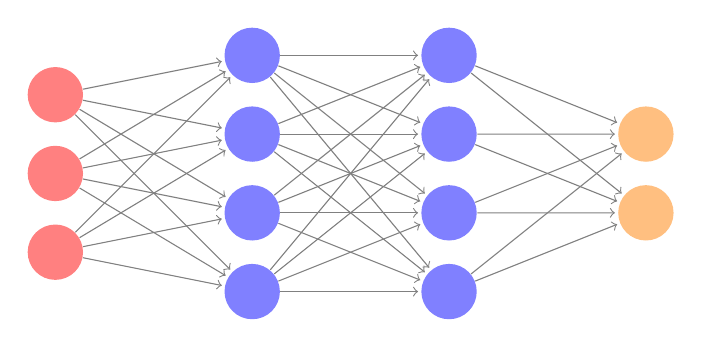
\begin{tikzpicture}[shorten >=1pt,->,draw=black!50, node distance=\layersep]
    \tikzstyle{every pin edge}=[<-,shorten <=1pt]
    \tikzstyle{neuron}=[circle, fill=black!25,minimum size=20pt,inner sep=0pt]
    \tikzstyle{input neuron}=[neuron, fill=red!50];
    \tikzstyle{output neuron}=[neuron, fill=orange!50];
    \tikzstyle{hidden neuron}=[neuron, fill=blue!50, minimum size=20pt];
    \tikzstyle{hidden neuron2}=[neuron, fill=blue!50, minimum size=20pt];

    \foreach \name / \y in {0,...,2}
        \node[input neuron] (I-\name) at (0,-\y) {};

    \foreach \name / \y in {0,...,3}
        \path[yshift=0.5cm]
            node[hidden neuron] (H1-\name) at (\layersep,-\y cm) {};

    \foreach \name / \y in {0,...,3}
        \path[yshift=0.5cm]
            node[hidden neuron2] (H2-\name) at (2*\layersep,-\y cm) {};    

    \foreach \name / \y in {0,...,1}
        % \node[output neuron,pin={[pun edge={->}]right:Output \#\y}, right of=H2-2] (O-\name) at (3*\layersep, -\y cm) {};
        \path[yshift=-0.5cm]
            node[output neuron] (O-\name) at (3*\layersep, -\y cm) {};


    \foreach \source in {0,...,2}
        \foreach \dest in {0,...,3}
            \path (I-\source) edge (H1-\dest);

    \foreach \source in {0,...,3}
        \foreach \dest in {0,...,3}
            \path (H1-\source) edge (H2-\dest);

    \foreach \source in {0,...,3}
        \foreach \dest in {0,...,1}
            \path (H2-\source) edge (O-\dest);
\end{tikzpicture}
\caption{Illustration of a fully connected feed-forward neural network with an input layer (red), two hidden layers (blue) and an output layer (orange).}
\label{fig:SimpleFFNN}
\end{figure}

Let $\boldsymbol{\theta} = \{ W_i, \boldsymbol{b}_i \}_{i = 1}^L$ represent the trainable parameters of the network in the parameter space $\mathcal{V}$, and $\mathcal{N}_{\boldsymbol{\theta}} : \mathbb{R}^{N_0} \to \mathbb{R}^{N_L}$ denote the realization of a neural network with $L$ layers, defined by
\begin{equation}
\begin{split}
    \mathcal{N}_{\boldsymbol{\theta}} &= \sigma_L \circ \mathcal{A}_L \circ \sigma_{L-1} \circ \ldots \circ \sigma_{1} \circ \mathcal{A}_1 \\
    &= \bigcirc_{i = 1}^L \sigma_i \circ \mathcal{A}_i.
\end{split}
\end{equation}
We call the parameters trainable, as we typically initialize them to random values, \textit{training} them through optimization with the help of the backpropagation algorithm.
We do this by measuring how well our model is able to predict a set of values with a cost function $\mathcal{C}$, which often gives the problem the form of finding
\begin{equation}\label{eq:argmintheta}
    \hat{\boldsymbol{\theta}} = \argmin_{\boldsymbol{\theta} \in \mathcal{V}} \mathcal{C} \left( \mathcal{N}_{\boldsymbol{\theta}}, \boldsymbol{x}, \boldsymbol{\hat{y}} \right),
\end{equation}
where $\boldsymbol{\hat{y}} \in \mathbb{R}^{N_L}$ are a set of target values.

A typical choice of $\mathcal{C}$ in a regression problem is the Mean squared error (MSE), defined by
\begin{equation}
    \frac{1}{n} \lVert \mathcal{N}_\theta(\boldsymbol{x}) - \boldsymbol{y} \rVert_2^2
    = \frac{1}{n} \sum_{i = 1}^n (\mathcal{N}_\theta(x_i) - y_i)^2.
\end{equation}



\subsection{Partial Differential Equations}
A Partial Differential Equation (PDE) is defined to be an equation containing a function with at least two different variables, as well as some degree of partial derivatives to these variables.
PDEs are ubiquitous in describing the properties, behavior, and evolution of physical systems.
A prime example is Poisson’s equation, which is of broad utility within theoretical physics. It is defined by
\begin{equation*}
    u_{xx} + u_{yy} = f,
\end{equation*}
where the residual $f$ is independent of $u$.

An important concept when discussing PDEs is differential operators.
A differential operator is defined as a function of the differentiation operator.
It is indeed a function from a function space $\mathcal{F}_1$ to another function space $\mathcal{F}_2$.
In the case of a function of $n$ variables $u(x_1, x_2, \ldots , x_n)$ the usual differential operator is defined as 
\begin{equation*}
    D^\alpha u = \frac{\partial u^{|\alpha|}}{\partial x_1^{\alpha_1} \partial x_2^{\alpha_2} \cdots \partial x_n^{\alpha_n}},
\end{equation*}
where $|\alpha| = \alpha_1 + \alpha_2 + \ldots + \alpha_n$.
When considering a function $u(x,y)$, we will denote $\frac{\partial u}{\partial x}$ as $u_x$, $\frac{\partial^2 u}{\partial x^2}$ as $u_{xx}$, $\frac{\partial u}{\partial y}$ as $u_y$ and so on.
We will when discussing general PDEs denote the differential operator characterizing the PDE by $\mathcal{L}$.
For example, for the Poisson equation mentioned above, we have $\mathcal{L}u = u_{xx} + u_{yy}$, and denote the equation as $\mathcal{L}u=f$.
We will also come across the differential operator $\nabla$ (nabla).
For a problem in three physical dimensions, nabla is defined as $\nabla = \frac{\partial}{\partial x}\boldsymbol{x} + \frac{\partial}{\partial y}\boldsymbol{y} + \frac{\partial}{\partial z}\boldsymbol{z}$, where $\boldsymbol{x},\boldsymbol{y},\boldsymbol{z}$ are the three-dimensional Euclidean unit vectors.

When considering time-dependent PDEs for physical problems, we require both initial- and boundary conditions.
Initial conditions are conditions for values at $t=0$, and boundary conditions are value conditions at the physical boundary of the problem.
In this paper we encounter Dirichlet-type boundary conditions (also referred to as first-type boundary conditions), that is when the value of the function on the boundary is given.
We return to the Poisson equation as an example;
we have for the function $u(x,y)$, $(x,y) \in [0,1]\times [0,1]$ the boundary conditions $u(0,y)=u(1,y)=u(x,0)=u(x,1) = 0$.
Another important is Neumann (or second-type) boundary conditions.
This is when the boundary conditions gives the value of the first order derivative of in the direction normal to the boundary.

\subsection{Physics-Informed Neural Networks}
Physics-Informed Neural Networks (PINNs) incorporate the PDE conditions directly into the Loss function of the network.
In doing so, we coerce the network into predicting results which adhere to the inherent physical laws.
In this way, we reduce the need for labeled data, and are able to be more confident in the predictions of our network.
Our neural network $\mathcal{N}_{\boldsymbol{\theta}}$ can then be regarded as an approximation of the hidden function $u$, notating it as $u^*$.
The cost function of the network can then be of the form of \autoref{eq:PINNloss}.
\begin{equation}\label{eq:PINNloss}
\begin{array}{rrrrr}
    C(\boldsymbol{x}, \boldsymbol{\theta}) =& & \frac{1}{N_{D}}\lVert u^* - \tilde{u} \rVert_2^2 &\leftarrow& \text{Data} \\
    &+& \frac{1}{N_{\Omega}}\lVert \mathcal{L}u^* - f \rVert_2^2 &\leftarrow& \text{PDE} \\
    &+& \frac{1}{N_{\partial \Omega}} \lVert u^*_{b} - g \rVert_2^2 &\leftarrow& \text{Boundary}.
\end{array}
\end{equation}

The total process of applying machine learning techniques can then be quite beneficial, as the process of accruing data, whether that be with measurements, numerically or analytically, can be extremely costly.
In addition, with a framework already set up, the process of setting up a PINN is quite simple, in contrast to developing a numerical algorithm.

The process of computing $\mathcal{L}u^*$ is done through automatic differentiation, detailed in \autoref{sec:JAX} and \autoref{sec:autodiff}.

Loss function, blablablabla. Trenger ikke target values, kan bare dunke på med PDE + boundary ogsånn. Sitering, har funket, har problemer, osvosvosv.

\subsection{Extended Physics-Informed Neural Networks}
Utvider Loss function, blablablabla Interface. Potensielle fordeler, ulemper, kompleksiteter osv.
